\documentclass{article}
%  \textheight		= 21cm
%  \textwidth		= 18cm
%  \topmargin		= -1cm
%  \oddsidemargin	= -1cm
\usepackage[spanish]{babel}
\usepackage[utf8]{inputenc}%%%Paquete para la acentuación, no hace falta poner \'vocal.
\usepackage{graphicx}
\usepackage{color}
\usepackage{import}
\usepackage{hyperref}

\setlength\parindent{0pt}
\renewcommand{\labelitemi}{$\diamond$}

\graphicspath{{resources/}}

\makeatletter
\newcommand{\logo}[2] {%
	\def\input@path{{#1}}
	\def\logoimg{#2}
}
\newcommand\version[1]{\renewcommand\@version{#1}}
\newcommand\@version{\@latex@error{No \noexpand\version given}\@ehc}
\makeatother

\begin{document}

\logo{resources}{LogoWariVicuna}
\version{ @LATEX_VERSION@ }
\title{Guía rápida del usuario}
\import{@CONFIG_PATH@/doxygen/}{title.tex}

\section{Introducción}
Wari es un sintonizador y reproductor de televisión digital que permite ver los canales de la TDA (Televisión Digital Abierta) y ejecutar aplicaciones Ginga.

\vspace{0.5cm}
El nombre Wari significa ``vicuña'' en Quechua y Aymara. La vicuña es un animal sagrado para las culturas del noroeste argentino, su lana es muy preciada, pero no se lo puede mantener en cautiverio porque no sobrevive. Wari es decididamente libre como el espíritu de este software.

\section{Usando Wari por primera vez}

Al ejecutar la aplicación por primera vez, la lista de canales estará vacía. Por lo tanto, se visualizará una imagen como la siguiente.

\vspace{0.5cm}
\centerline{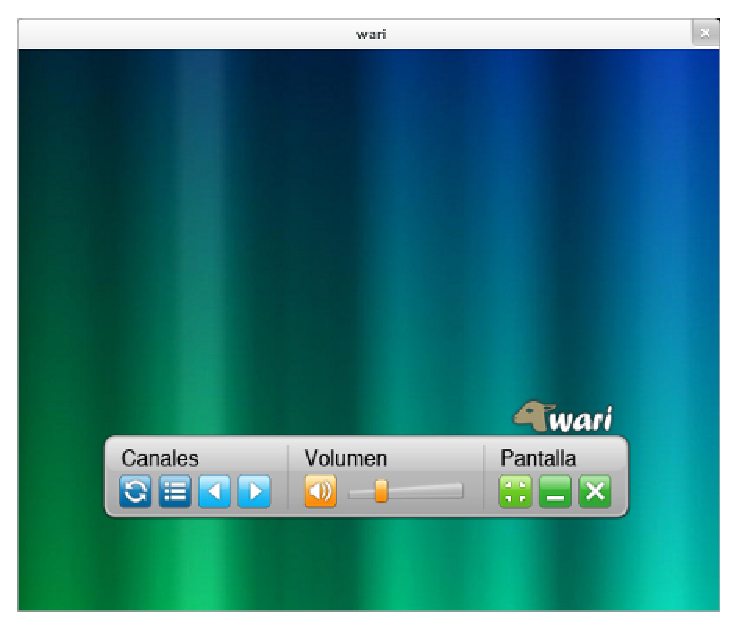
\includegraphics[scale=1,keepaspectratio=true]{inicio}}

\vspace{0.5cm}
Al presionar el botón 
\includegraphics[scale=0.5,keepaspectratio=true]{BtnCanalesScan} ``Buscar Canales'' para poder sintonizar la TDA (Televisión Digital Abierta). Una barra de progreso aparecerá en la pantalla indicando el estado de la búsqueda de canales.

\vspace{0.5cm}
\centerline{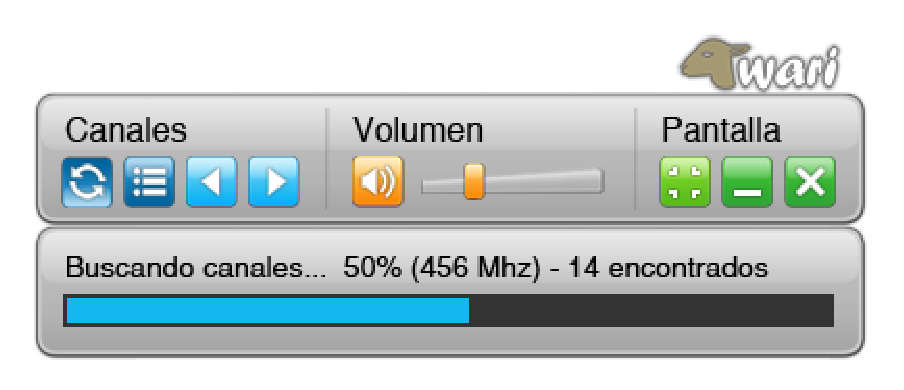
\includegraphics[scale=0.75,keepaspectratio=true]{Player-Scan}}

Una vez que la búsqueda finaliza, la barra de progreso desaparece y se sintoniza el primer canal encontrado.

El panel de control principal se puede ocultar o visualizar, haciendo un clic con el botón izquierdo del mouse en cualquier lugar de la pantalla o presionando la tecla ``c'' del teclado.

\vspace{0.5cm}
\section{Panel de control principal}

\centerline{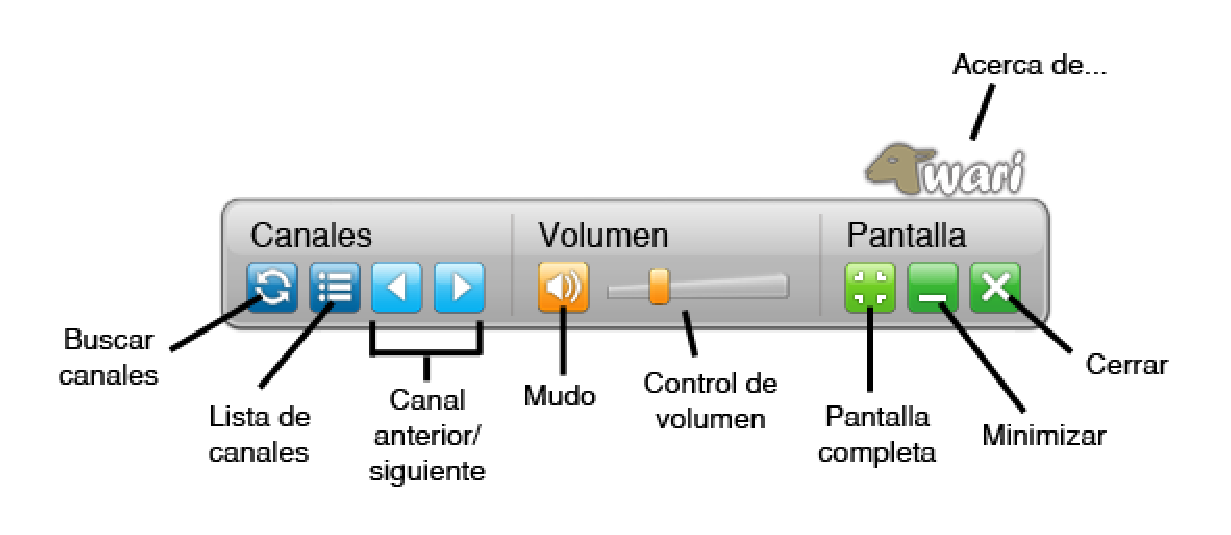
\includegraphics[scale=0.75,keepaspectratio=true]{Player-Referencias}}

\vspace{0.5cm}

\textbf{Canales:}
\vspace{0.5cm}


\includegraphics[scale=0.75,keepaspectratio=true]{BtnCanalesScan} \textbf{Buscar canales:} Busca canales y los agrega a la lista de canales.


\includegraphics[scale=0.75,keepaspectratio=true]{BtnCanalesLista} \textbf{Lista de canales:} Muestra / oculta la lista de canales.

\centerline{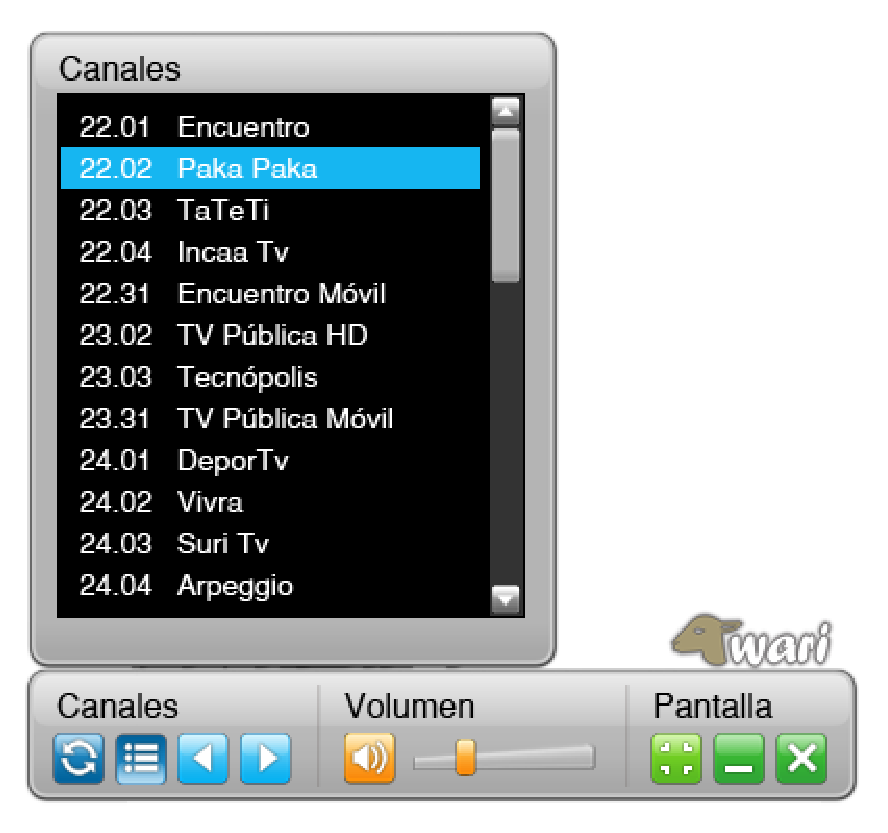
\includegraphics[scale=0.75,keepaspectratio=true]{ListaCanales}}

\vspace{0.5cm}
La lista de canales se puede navegar usando el mouse o el teclado.

Con el teclado, los botones cursor arriba, cursor abajo y el $<$Enter$>$ permiten sintonizar el servicio seleccionado.

\vspace{0.5cm}

\includegraphics[scale=0.75,keepaspectratio=true]{navAntSig} \textbf{Canal anterior y siguiente:} permite sintonizar el canal anterior o el siguiente de la lista de canales. También se pueden usar las teclas cursor izquierda y cursor derecha para la misma funcionalidad.

\vspace{0.5cm}
\textbf{Volumen:}

\vspace{0.5cm}

\includegraphics[scale=0.75,keepaspectratio=true]{BtnVolumen} El botón de mudo permite silenciar el audio y volver a escucharlo, y el control de volumen permite subir y bajar el volumen del audio.
	
\vspace{0.5cm}	
\centerline{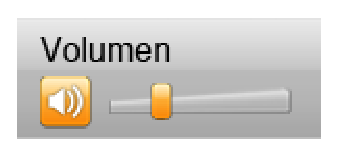
\includegraphics[scale=0.75,keepaspectratio=true]{BtnVol}}

\vspace{0.5cm}
\textbf{Pantalla:}

\vspace{0.5cm}

\includegraphics[scale=0.75,keepaspectratio=true]{BtnPantallaCompleta} \textbf{Pantalla Completa:} Permite que la imagen de video ocupe toda la pantalla.


\includegraphics[scale=0.75,keepaspectratio=true]{BtnPantallaMinimizar} \textbf{Minimizar:} Mueve 			la ventana a la barra de tareas.


\includegraphics[scale=0.75,keepaspectratio=true]{BtnPantallaCerrar} \textbf{Cerrar:} Cierra la 			aplicación

\vspace{0.5cm}
\textbf{Acerca de...}

Haciendo un clic sobre el logo del panel principal de la aplicación, se abre una ventana 			indicando la versión y un texto descriptivo de la misma.

\vspace{0.5cm}
\centerline{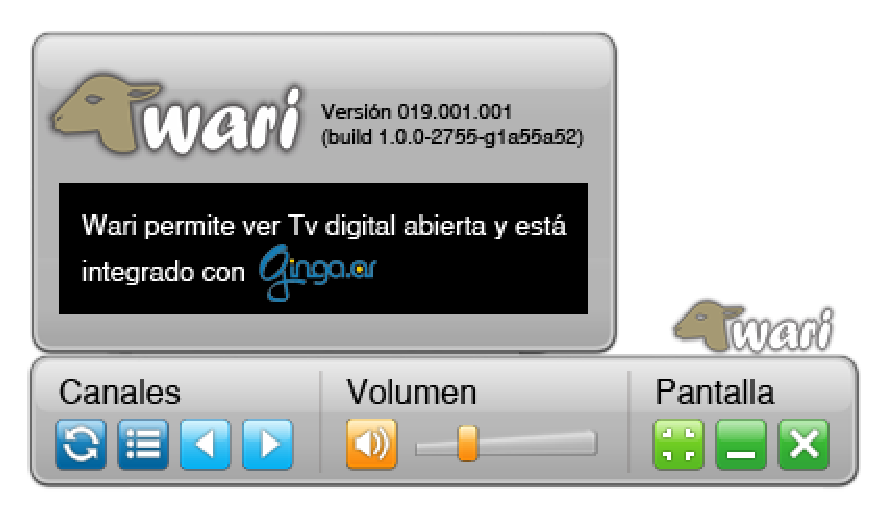
\includegraphics[scale=0.75,keepaspectratio=true]{About}}

\vspace{0.5cm}
\section{Atajos de teclado}
Wari puede usarse mediante el teclado sin necesidad de tener a la vista el Panel de control principal.

Los atajos de teclado son:

\begin{itemize}
	\item \textbf{r:} Buscar canales
	\item \textbf{l:} Lista de canales
	\item \textbf{z (y flecha izquierda):} Bajar un canal
	\item \textbf{q (y flecha derecha):} Subir un canal
	\item \textbf{m:} Mudo / No Mudo	
	\item \textbf{w:} Subir volumen
	\item \textbf{x:} Bajar volumen
	\item \textbf{f y doble clic con el mouse:} Pantalla completa / restaurar
	\item \textbf{i:} Mostrar / ocultar menu de acerca de... (teniendo activado el panel principal)
	\item \textbf{c y clic del mouse:} Mostrar / ocultar Panel de control
	\item \textbf{s:} Activar / desactivar subtitulos
	\item \textbf{a:} Cambiar de audio (si hay más de uno disponible)
\end{itemize}

\section{Aplicaciones interactivas}

Para poder visualizar las aplicaciones Ginga, se debe tener instalado Ginga.ar\footnote{Disponible en: \url{http://tvd.lifia.info.unlp.edu.ar/ginga.ar/}}

Si la señal sintonizada contiene una aplicación interactiva, ésta se descargará automáticamente mostrando una barra de progreso. 

\vspace{0.5cm}
\centerline{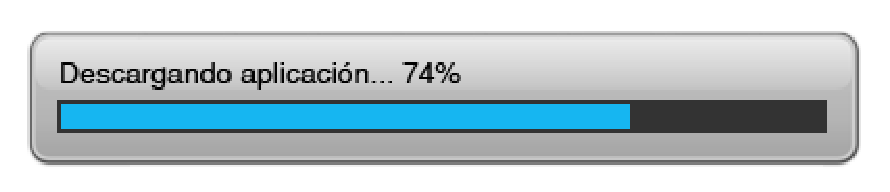
\includegraphics[scale=0.85,keepaspectratio=true]{DescargandoApp}}

\vspace{0.5cm}
Una vez descargada, el usuario puede interactuar con la misma usando las teclas $<$Fn$>$.

Cada $<$Fn$>$ tiene una función específica que dependerá de la aplicación con la que se esté interactuando en el momento.
\begin{itemize}
	\item \textbf{F1:} Rojo
	\item \textbf{F2:} Verde
	\item \textbf{F3:} Amarillo
	\item \textbf{F4:} Azul
	\item \textbf{F5:} Menú
	\item \textbf{F6:} INFO (normalmente abre la aplicación cuando se muestra el botón info en la pantalla, y 	minimiza la aplicación sin cerrarla volviendo al botón info cuando la aplicación está desplegada)
	\item \textbf{F10 / Esc:} Cierra la aplicación interactiva Ginga, si esta en ejecución.
\end{itemize}

\end{document}
